\section{Core network}
\label{sec:core}

Based on the mobile network scope, the core can be characterized as the most critical element in the 5G system. 3GPP Release 15~\cite{3gpp:rel15nr21.915} defined the core as a set of components interconnected by a service layer. Each component has a specific set of responsibilities for consuming and providing services to/from other elements of the 5G system, through Application Programming Interface (API) defined by the standard. The structure of the software components and their interconnections via APIs is shown in Fig.~\ref{5GCore}. Release 15 introduced substantial changes in the way mobile networks are designed to support a wide range of services, each as distinct performance requirements~\cite{foukas2017network}.

\begin{figure}[hbt]  
 \begin{center}
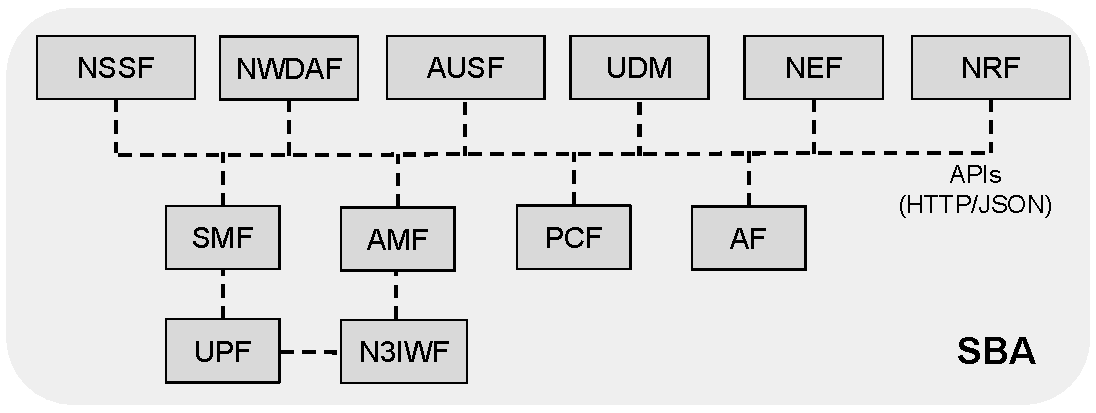
\includegraphics[width=0.5\textwidth]{figs/5G-Core.pdf}
  \end{center}
\caption{Core 5G software components.}
\label{5GCore}
\end{figure}

Given the 5G core relevance, each of the elements that compose the core needs to be robust, resilient, highly available, and scalable. These characteristics are usually associated with the cloud computing concept. In the Release 15 context, each of the components that compose the new 5G core can be split into Virtual Network Functions (VNFs). In this way, each VNF can be available on-demand in a cloud infrastructure. The use based on the split of VNF is possible because physical interfaces like in previous architectures do not interconnect the components end-to-end. Instead, each of the components of the core must expose a set of software functionalities through SBA~\cite{karnouskos2012SOA}. In this context, each VNF offers one or more services for other VNFs. Considering the new definition of the SBA model, the exposure of functions applies only to the signaling context and not to the transfer of user data.

One of the communication methods used for an SBA is based on Representational State Transfer (REST) over HyperText Transfer Protocol (HTTP). This method consists of a set of rules and guidelines, widely used in the interconnection of distributed systems. The rules define how communication technologies on the Web access services through the use of APIs. The 3GPP expectation as this initiative is to make the task of extending the network resources simpler. Another aspect regarding the communication mechanism is that it should be seen as a logical option since the components specification for VNFs assumes that these components are running in a virtualized environment~\cite{imadali2018NFV}. 

The components of the 5G core can be seen as an interconnected network of services. Each VNF of a component performs specific responsibilities and interconnects with other VNFs producing and consuming services. The main characteristics of each of these components are discussed in the following subsections. We briefly describe the main components of the 5G core without the objective of listing all or making an exhaustive presentation. The complete list of components and their detailed description requires hundreds of pages of the standard or a whole book on it~\cite{hedman20195g}.


\subsection{Main Components}

In this subsection, we introduce the components needed to create a basic 5G core. In this way, we have named these components of main.

\subsection*{Access and Mobility Management Function (AMF)}

Mobility can be considered the essence of a 5G system. The mobility management begins when a new connection is established between a UE and the core of the network. This action triggers a set of procedures to identify UE, providing a security structure to offer a transport channel of messages. The main goal of the AMF component is to ensure that the communication process occurs cohesively and transparently, considering user mobility as a critical factor. Based on the functions implemented in AMF, the network can reach a specific user to notify about any messages or calls received, for example. Moreover, the AMF component can allow a particular UE to initiate a communication process with other UEs connected to RAN or with Internet access. Another fundamental functionality of AMF is to guarantee the connectivity holding the existing sessions when UEs move between different access points.

In 5G networks, there is a need to provide flexible support for a wide range of new users~\cite{foukas2017network}. Many of these users have specific requirements concerning mobility. For example, a particular UE used in a factory does not usually move, while UE in an autonomous vehicle or remotely controlled can present high mobility. To better support these different needs, 3GPP Release 15~\cite{3gpp:rel15nr21.915} splits the mobility procedures into three categories for the AMF component:

 \begin{itemize}
  \item Standard procedures can be characterized as a set of steps running when any UE requests a connection to the core. Among these steps, the security process is highlighted, composed of primary authentication, management of access keys, identification, and basic configuration of UE.
  \item Specific procedures have the function of managing the registration and periodic updating of the mobility of a given UE in AMF. Moreover, these procedures control the closing of the UE registration, provide scope for different access technologies. 
  \item Connection Management procedures are used to establish a secure communication process between a given UE and the core. Moreover, this procedure works when a specific UE needs to carry out a network resource reservation process for sending data.
\end{itemize}

Each of these categories of procedures aims to provide UEs with functionalities to establish connections with the core network, using the services associated with mobility.


\subsection*{Session Management Function (SMF)} 

The SMF component is responsible for managing the UE sessions, \textit{i.e.}, the sessions representing the connected users. The main responsibilities of SMF are activities of establishing, modifying, and releasing the individual sessions of UEs and allocating the IP address for each connected UE. However, the communication between UEs and SMF is performed indirectly through the AMF component. The function of AMF forwards the messages associated with the session of a given UE and the functions of the SMF component.

The SMF component's internal functions interact with VNFs of the other components through the producer/consumer model, defined regarding the SBA~\cite{karnouskos2012SOA}. For example, SMF is responsible for controlling different functions associated with the UPF component. This control includes the SMF's ability to configure the direction of data traffic associated with a UPF for a given UE session. Moreover, SMF must run monitoring and control actions on UPF. The SMF component interacts with functions related to PCF, aiming to execute the session policy of the UEs connected. This execution action can be described as one of the main tasks associated with a 5G system. For instance, this action determines the guidelines for data connectivity between a UE and the Data Network (DN).


\subsection*{User Plane Function (UPF)}

3GPP Release 15~\cite{3gpp:rel15nr21.915} introduces the UPF component as a fundamental function within the new SBA model. UPF can be seen as part of a split process between CP and UP, initially introduced in the Release 14~\cite{3gpp:rel14nr133.185} with CUPS. Decoupling data and control allows the SBA model to decentralize its components further. For example, it can direct activities such as packet processing to be placed closer to the edge network, increasing QoS for the user, and reducing network traffic.


SMF controls the functionalities implemented in the UPF component. The main function of UPF is associated with the forwarding and the data processing from UEs. This component is also responsible for generating notifications related to data traffic and the inspection of packets. UPF also works as a stable interconnection point between the core and any external networks. Moreover, UPF allows communication to happen transparently, hiding complex aspects associated with mobility. IP packets destined to a given UE are forwarded (from the Internet) to the respective UPF, which is attending that UE, even when UE is on the move. In general, the UPF component is responsible for:

\begin{itemize}
  \item Design the rules for the interconnection point between the core and any external networks;
  \item Serve as an external access point for Protocol Data Unit (PDU), interconnecting different data networks;
  \item Forward and route the packets and inspect these packets aiming to detect application characteristics;
  \item Apply the definitions associated with the management of the user data plane and provide information on the data traffic. 
\end{itemize}
 
 
\subsection*{Authentication Server Function (AUSF)}

AUSF is responsible for the authentication service of UEs through the access credentials provided by UDM. Moreover, AUSF provides services associated with the encryption for allowing secure information traffic and the execution of the roaming update processes, as well as other parameters related to UE.

Generally, the AUSF component provides services consumed by AMF functions, which request resources associated with the authentication process. For example, AUSF internally processes the requests of functions of the AMF component and after delegates to services provided by the UDM component to run the registry procedures in the data repository.

\subsection*{Unified Data Management (UDM)} 

The UDM component manages the users' data on the network in an only centralized element. UDM is similar to the HSS of the EPC core of the 4G networks. Through UDM, several VNFs of the SBA model can run many actions, such as registration and authentication of UEs, user identification, application of access rules and authorization, etc. The UDM component interacts directly with AMF, which forwards the requests from other components. Moreover, in scenarios where exist more than one instance of the AMF component on the network, UDM must control which instance is responsible for serving a given UE~\cite{toskala20205}. Among the UDM functionalities, we can highlight~\cite{etsiTS:123501}:

\begin{itemize}
    \item Generation of the Authentication and Key Agreement;
    \item Handling user identification;
    \item Support for privacy-protected signature identifier hiding;
    \item Access authorization based on the signature data (\textit{e.g.}, restrictions associated with mobility)
    \item Signature management;
    \item SMS management.
\end {itemize}

The UDM component works as a front-end for the user's subscription data recorded in the Unified Data Repository (UDR). UDM employs this subscription data to execute the logic of several applications, such as access authorization, registration management, and accessibility for finalizing events. UDR is a database where several types of data are stored, and the access is offered as a service to other components such as UDM, PCF, and NEF. There is an optional storage component called Unstructured data storage function (UDSF), which allows other components or functions to record dynamic context data outside the function or component itself. In the 3GPP context, unstructured data refers to the structure is not defined in the specifications, allowing each provider to use a give UDSF and choose its appropriate structure for storage. There is no requirement for any access compatibility or data storage in UDSF from different providers. 


\subsection*{Network Repository Function (NRF)}

The NRF component is the repository, where all the functions available for a given network are listed. The goal of this component is to allow VNFs can find the appropriate function to meet their requirements. NRF has the responsibility to select the most suitable service provider component based on the performance criteria provided. In this way, the NRF component is updated whenever a new NBF instance is deployed or modified. Moreover, NRF holds information on the other VNFs, such as type, capacity, address, etc.

Based on the SBA scope, the NRF component plays a fundamental role in the functioning of the other VNFs. This component offers a central mechanism that allows automating the configuration process necessary for the other VNFs to discover and connect to specialized services. 


\subsection{Additional Components}

In this subsection, we present additional components of the 5G core. These components are fundamental for creating a complete infrastructure of network functions for providing several business opportunities.



\subsection*{Policy Control Function (PCF)}

This component performs the same function as PCRF of the EPC core in the 4G system. PCF is responsible for controlling the behavior of the network, applying security and control rules, related to session management, mainly for functionalities associated with user mobility. This component interacts directly with AMF, providing an access and mobility policy that can add the control of access restrictions to services in a given area, for example. Moreover, PCF can include the management of topics associated with priority access to the channel of given UEs to the detriment of others. This management is named Radio Frequency Selection Priority (RFSP).

In the session management context, PCF can interact with the application functions and SMF. The main goal is to provide metrics associated with QoS and information regarding the data flow, which is obtained by regularly monitoring events related to the PDU session. Moreover, PCF offers security policy information for UEs. These policies can be associated with network resources and rules for selecting resource slicing. For example, PCF can be triggered to provide information when a given UE performs an access selection (UE access selection) or when a PDU session is established~\cite{hedman20195g}. The interaction between PCF and the other application functions is implemented through the exposure of six services, namely:

\begin{itemize}
\item \textit{PCF-AM-PolicyControl} -- provides information on access control policies, network selection, mobility management, and guidelines for the selection of routes between UEs and AMFs;
\item \textit{PCF-PolicyAuthorization} -- supplies authorization and provides access control policies to a request for an AF element, related to the PDU session in which AF is associated;
\item \textit{PCF-SM-PolicyControl} -- provides to SMF component guidelines for access related to PDU session in which the component is associated;
\item \textit{PCF-BDT-PolicyControl} -- supplies a set of guidelines for the NEF component to be used by applications to transfer data in the background plane;
\item \textit{PCF-UE-PolicyControl} -- provides control guidelines to be used in the communication process management between UEs and other network functions;
\item \textit{PCF-EventExposure} -- allows other network functions to register to be notified when a given event happens.
\end{itemize}

The decision on the application of the monitoring and control policies made by PCF is based, in part, on analytical information provided by other network functions, such as NWADF. Moreover, PCF is a fundamental component in a scenario where an AF needs to perform a given activity, \textit{i.e.}, data transfer in the background plane. In this case, AF can contact PCF to infer the best time interval for the activity's execution. This behavior allows the system operator to offer information to application providers about the most appropriate time to transfer data in the background plane.


\subsection*{Network Slice Selection Function (NSSF)}

In the context of the 5G networks, Network Slicing can be defined as a possibility for the system operator to allocate a resource set (in general, virtualized), to meet the requirements of given services or applications~\cite{7784887}. The aim is to offer support for a wide range of services, each with specific performance demands~\cite{foukas2017network}. The virtual resource slices are logical instances of network resources needed to meet a given request. A slice can include RAN and core resources, and even extrapolate to transport networks between several RANs and cores, considering network the end-to-end network service.


The 5G core architecture defines the NSSF component as being responsible for managing the available network slice instances. This component selects the network slice instances and the set of AMFs available for a given UE. AMF can be a component dedicated to a specific slice or to serve a set of network slice instances. The NSSF function is to assist AMF in choosing the available network slices, redirecting traffic between the controlled network slices. Moreover, NSSF can be seen as an orchestrator that can influence how network traffic is routed. This component produces two services, a selection service that provides information about the selected network slice and another availability service that generates information concerning the available resource slices.


\subsection*{Network Exposure Function (NEF)}

The NEF component is responsible for exposing some internal events related to UEs and the SBA model. The exhibition of these events aims to meet the demand for specific applications and VNFs of other components. For example, these demands need to access to the location or notify about the connectivity interruption of a given UE. Moreover, this information allows the AMF component to adjust the system according to user group behavior.

The possibility of exposing internal events through a NEF access interface opens new business opportunities for service providers, allowing in some cases, more advanced services to be offered by third parties. For example, an application can use the functions exposed by the NEF component to know if a given UE is accessible or not. Moreover, these functions can determine the geographical location of UE or if its device is in the movement. The NEF component responds to requests from several VNFs through regular interactions between UDM and AMF components.


\subsection*{Network Data Analytics Function (NWDAF)}

NWDAF is an optional component in the core architecture and is responsible for collecting several types of information from the network and its users. This information is later organized and analyzed to provide the inferred results for other network functions. The description of this component was written superficially in Release 15~\cite{3gpp:rel15nr21.915}, and its detailed specification is expected for Release 16.

The data collected by NWDAF comes from several other network functions that compose the core. The data collection is made through the services layer that connects the core components via the writing service. This service can be activated by the internal events triggered by each component. Moreover, NWDAF collects information about the operation of the system and data registry information in the UDR component.

Based on the specification, the services provided by NWDAF can be consumed by any core component. The external access is also possible using the NEF component. The analyzes made by NWDAF on the data collected over time can be used as a historical and statistical resource to predict future values. Moreover, the analytical data produced by NWDAF can be used to apply specific actions in the network context.

\subsection*{\textit{Application Function} (AF)}

AF is a generic component that represents a possible application, internal or external, to the operator's network, which interacts with the SBA model. The interaction process of AFs with SBA can influence some aspects of the whole system. For example, an AF can interact with the PCF component through services exposed by the NEF component, improving QoS aspects and, consequently, the charging and pricing policies.

An essential factor that must be evaluated by the system operator is the confidence degree that an AF component can have to interact directly with specific VNFs. For example, an AF with higher reliability can access VNFs from all components of the SBA model, directly. At the same time, a lower reliable AF must first interact with the NEF component before accessing more sensitive network functions. 

\subsection*{Non-3GPP InterWorking Function (N3IWF)}

The N3IWF component is used to integrate non-3GPP accesses with the 5G core. WiFi (IEEE 802.11) and Data Over Cable Service Interface Specification (DOCSIS) are examples of non-3GPP access technologies intended for integration by the standard. The conventional 3GPP access uses a BS, \textit{e.g.}, eNB (4G) or gNB (5G). However, the non-3GPP access starts on a different device, for example, a WiFi access point or a Hybrid fiber-coaxial (HFC) modem. This device uses the N3IWF component to access the 3GPP network and other 5G core components.

All traffic from the N3IWF component is sent through secure channels, and it is isolated from all 3GPP traffic. The isolation is maintained not only for data traffic (usual for 3GPP communications) but also for control traffic, including the traffic before the authentication process. More details about the N3IWF component, with its use and the interaction with other SBA components, are described in Subsection~\ref{subsec:nao-3GPP}.


\subsection{5G core demonstration}\label{sec:demo_nucleo}

\subsection*{Goals}

The main goal of this demonstration is to present in a practical way the main functionalities of the 5G core based on the SBA model. Moreover, we comment on the installation and configuration processes of software that implements the 5G core, providing material to replicate this demonstration.


\subsection*{Description}

In this demonstration, we use the 5G core based on the open-source SBA model. We also present how to emulate RAN and multiple UEs. The presentation is organized in two experiments: (1) UEs, RAN, and core, all implemented in software; (2) UE in hardware (conventional mobile phone), eNodeB in hardware (SDR) and software, and the 5G core implemented in software. All components are implemented using Docker containers that can be hosted on a cloud infrastructure. Fig.~\ref{fig:demo2} shows the software and hardware components that are used in the 5G core demonstration.

\begin{figure*}[htb] 
 \begin{center}
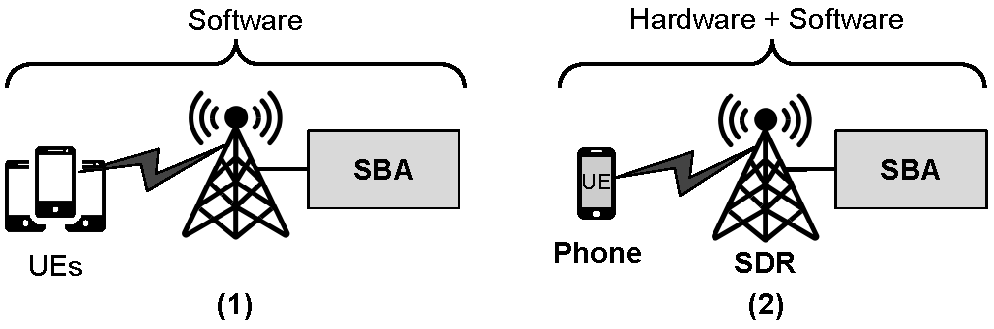
\includegraphics[width=0.6\textwidth]{figs/demo2-en.pdf}
  \end{center}
\caption{Experiments with a 5G core.}
\label{fig:demo2}
\end{figure*}


\subsection*{Additional information}

During the tutorial, we present demonstration videos of the experiments. Moreover, the manuals are available with details on how the practices can be replicated. Finally, containers and any extra source code produced by the team and need to replicate the experiments are publicly available.


Repository for this tutorial:\\
\url{https://github.com/LABORA-INF-UFG/NetSoft2020-Tutorial4}.


